\newpage

\section{Вычислительный эксперимент}
\subsection{Кластеризация точек временного ряда}
Для анализа свойств предложенного алгоритма кластериизации был проведен вычислительный эксперимент в котором кластеризация точек временного ряда проводилась используя матрицы попарных расстояний~$(\ref{eq:cl:9})$.

В качестве данных использовались две выборки временных рядов, которые описаны в таблице~\ref{table_1}. 
Выборка Physical Motion это реальные временные ряды полученные при помощи мобильного акселерометра. 
Синтетические временные ряды были построены при помощи нескольких первых слагаемых ряда Фурье со случайными коэффициентами из стандартного нормального распределения. 
Генерация данных состояла из двух этапов. 
На первом этапе генерировались короткие сегменты~$\textbf{v}$ для построения множества~$\mathbf{V}$. 
Вторым этапом генерации выборки~$\textbf{x}$ является следующим случайным процессом:
\begin{equation}
\label{eq:exp:1}
\begin{aligned}
\textbf{x} = [\textbf{v}_{1}, \textbf{v}_{2}, \cdots, \textbf{v}_{M}] + \bm{\varepsilon}, \quad \begin{cases}
    \textbf{v}_{1} \sim \mathcal{U}\left(\mathbf{V}\right),\\
    \textbf{v}_{i} = \textbf{v}_{i - 1}, & \text{с вероятностью}~\frac{3}{4}\\
    \textbf{v}_{i} \sim \mathcal{U}\left(\mathbf{V}\right), & \text{с вероятностью}~\frac{1}{4}
\end{cases},
\end{aligned}
\end{equation}
где~$\mathcal{U}\left(\mathbf{V}\right)$~---~равномерное распределение на объектах из~$\mathbf{V},$ а $\bm{\varepsilon}$ является шумом из нормального распределения.

\begin{table}[h!t]
\begin{center}
\caption{Описание временных рядов в эксперименте кластеризации точек временного ряда}
\label{table_1}
\begin{tabular}{|c|c|c|c|}
\hline
	Ряд,~$\textbf{x}$ &Длина ряда,~$N$& Число сегментов,~$K$&Длина сегмента,~$T$\\
	\hline
	\multicolumn{1}{|l|}{Physical~Motion~1}
	& 900& 2& 40\\
	\hline
	\multicolumn{1}{|l|}{Physical~Motion~2}
	& 900& 2& 40\\
	\hline
	\multicolumn{1}{|l|}{Synthetic~1}
	& 2000& 2& 20\\
	\hline
	\multicolumn{1}{|l|}{Synthetic~2}
	& 2000& 3& 20\\
\hline

\end{tabular}
\end{center}
\end{table}

\begin{figure}[h!t]\center
\subfloat[]
{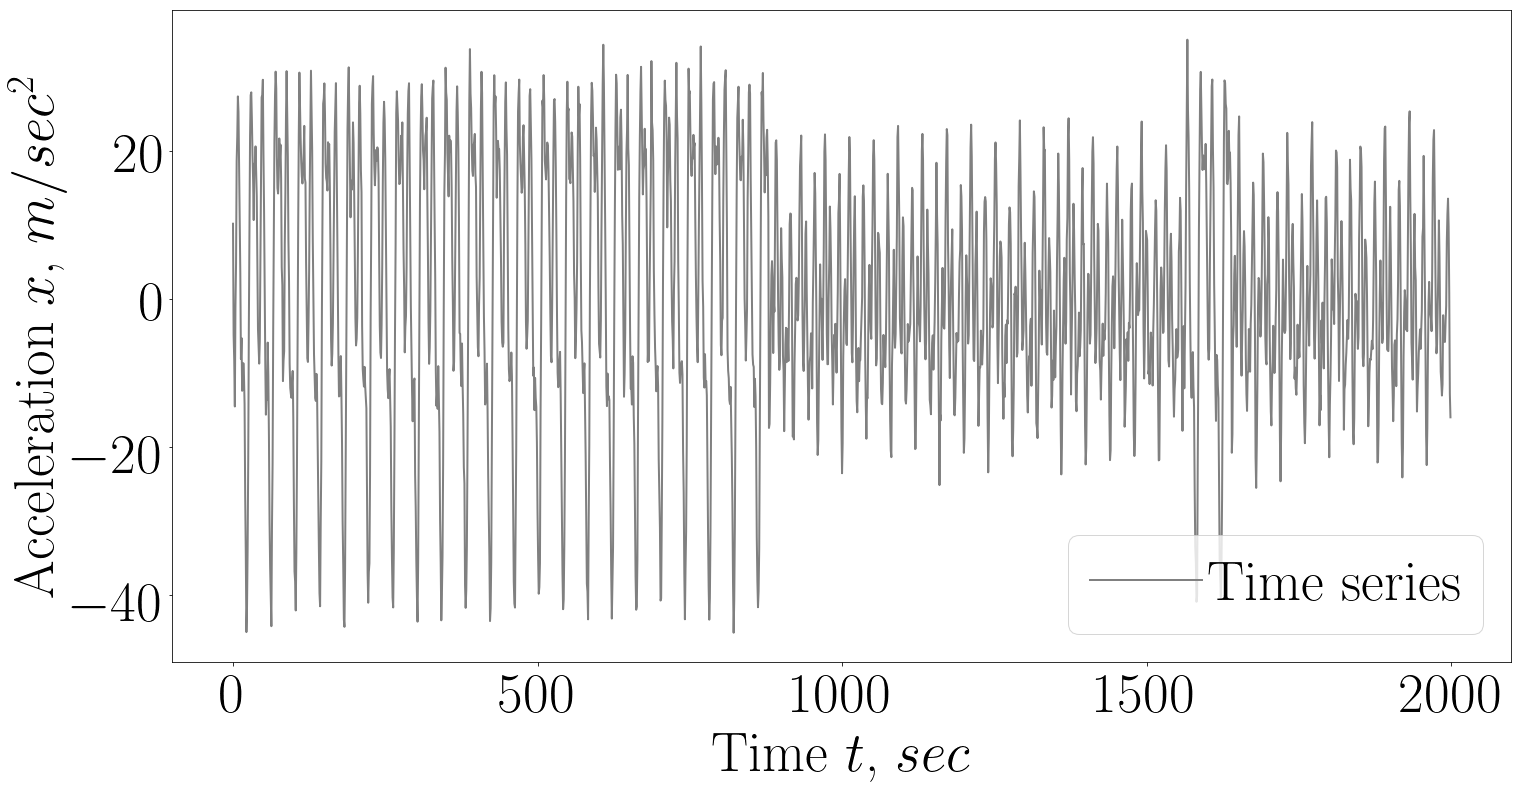
\includegraphics[width=0.5\textwidth]{results/2_patern_2_series}\label{fig_synthetic_series_2}}
\subfloat[]
{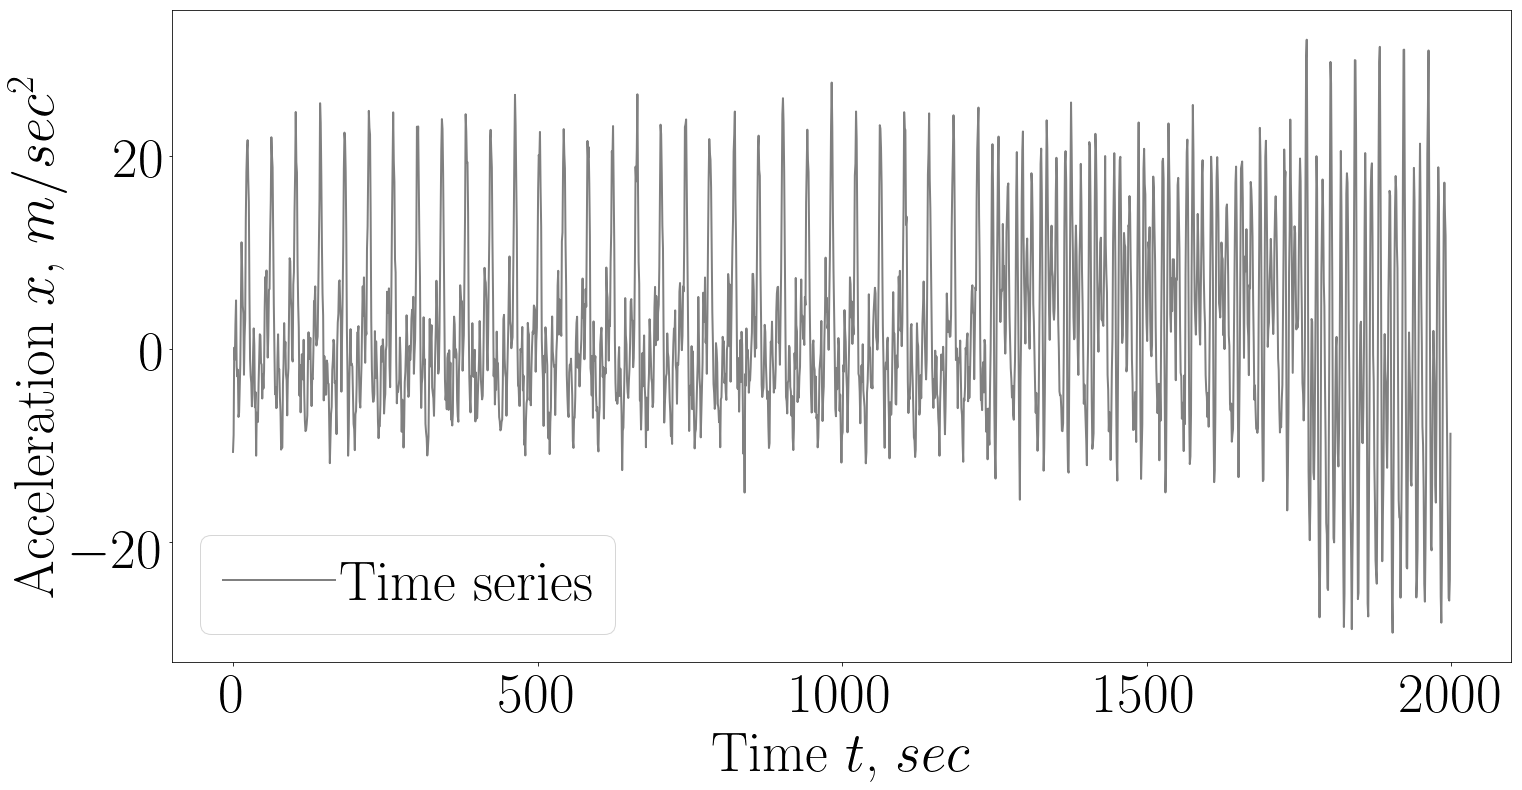
\includegraphics[width=0.5\textwidth]{results/3_patern_2_series}\label{fig_synthetic_series_3}}\\
\caption{Пример синтетически построенных временных рядов: a) для временного ряда Synthetic~1; b) для временного ряда Synthetic~2}
\label{fig_synthetic_series}
\end{figure}

\begin{figure}[h!t]\center
\subfloat[]
{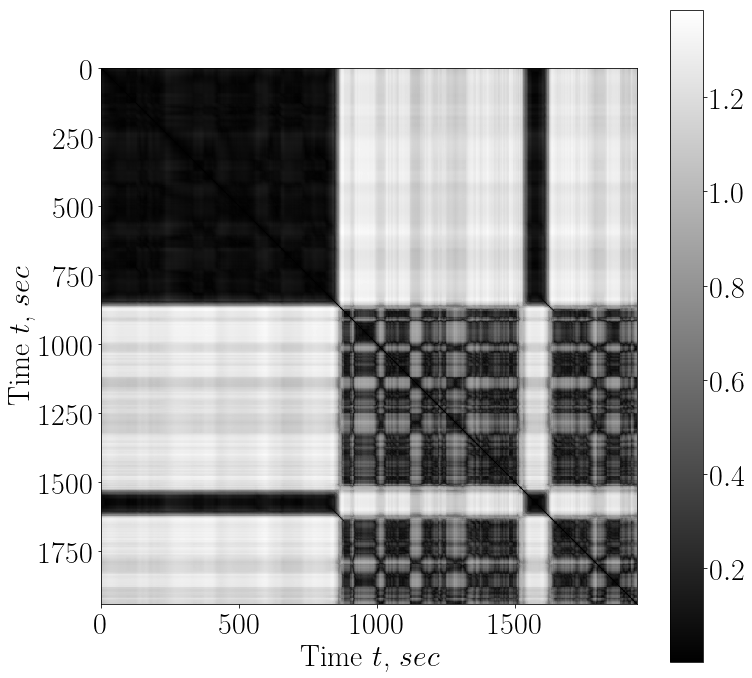
\includegraphics[width=0.5\textwidth]{results/2_patern_2_full}}
\subfloat[]
{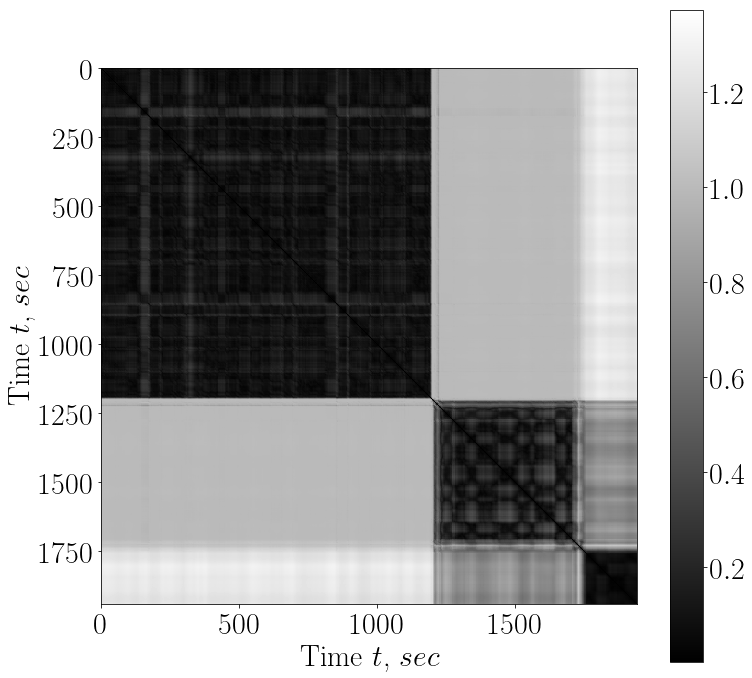
\includegraphics[width=0.5\textwidth]{results/3_patern_2_full}}\\
\caption{Матрица попарных расстояний~$\textbf{M}$ между точками временного ряда: a) для временного ряда Synthetic~1; b) для временного ряда Synthetic~2}
\label{fig_synthetic_distance}
\end{figure}

\begin{figure}[h!t]\center
\subfloat[]
{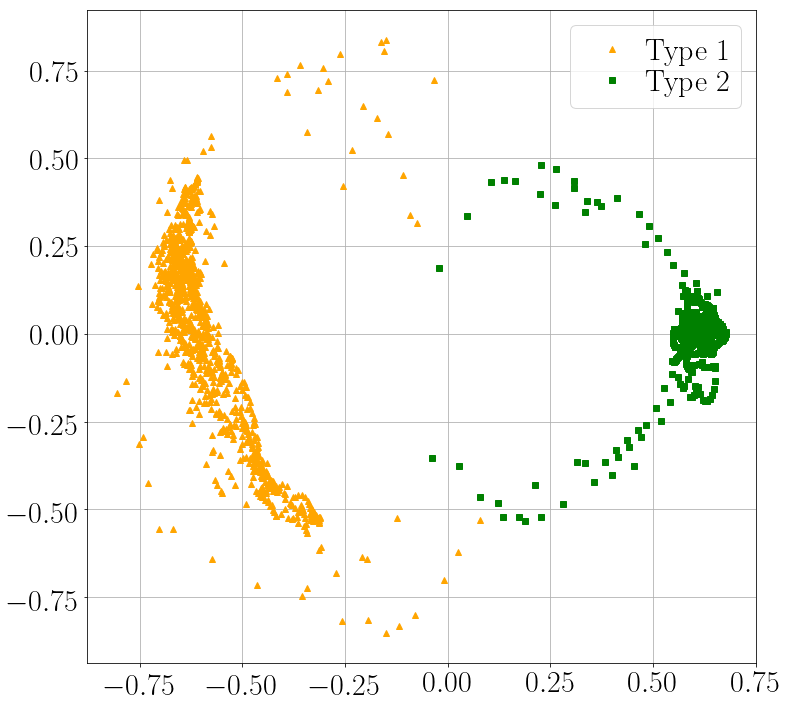
\includegraphics[width=0.5\textwidth]{results/2_patern_2_2D_vector}}
\subfloat[]
{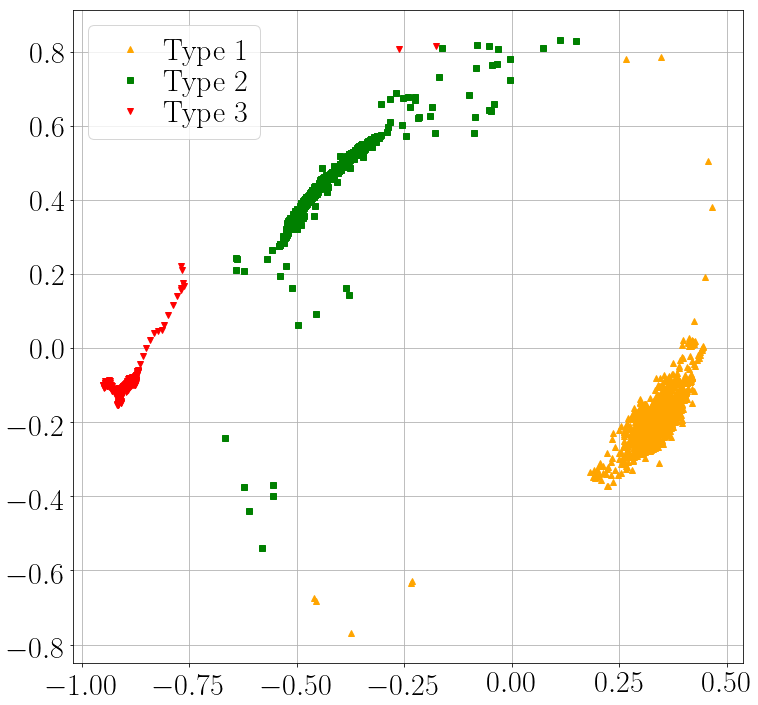
\includegraphics[width=0.5\textwidth]{results/3_patern_2_2D_vector}}\\
\caption{Проекция точек временного ряда на плоскость при помощи матрицы попарных расстояний~$\textbf{M}$: a) для временного ряда Synthetic~1; b) для временного ряда Synthetic~2}
\label{fig_synthetic_2D}
\end{figure}

\begin{figure}[h!t]\center
\subfloat[]
{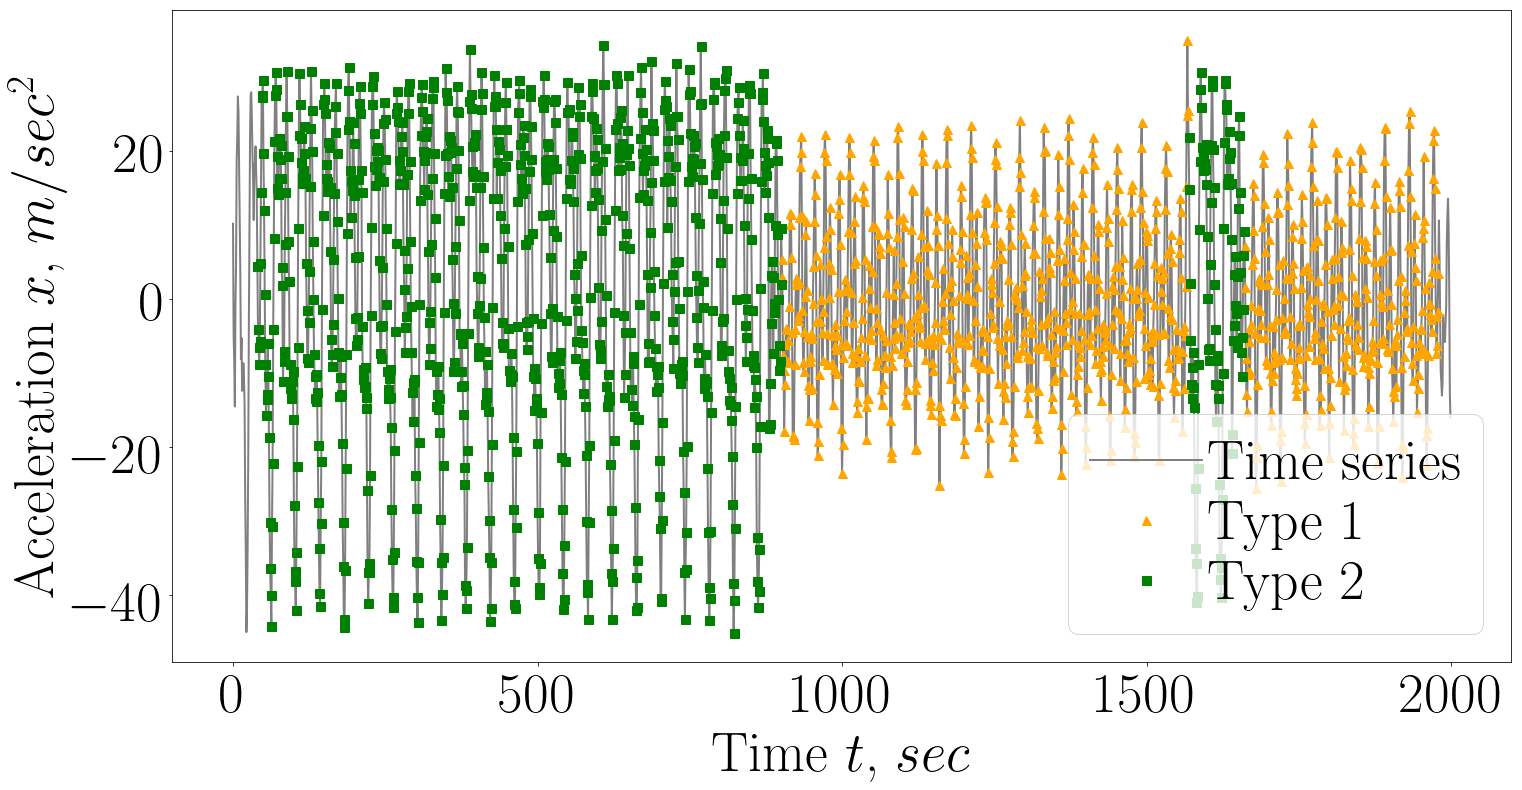
\includegraphics[width=0.5\textwidth]{results/2_patern_2_claster_vector}}
\subfloat[]
{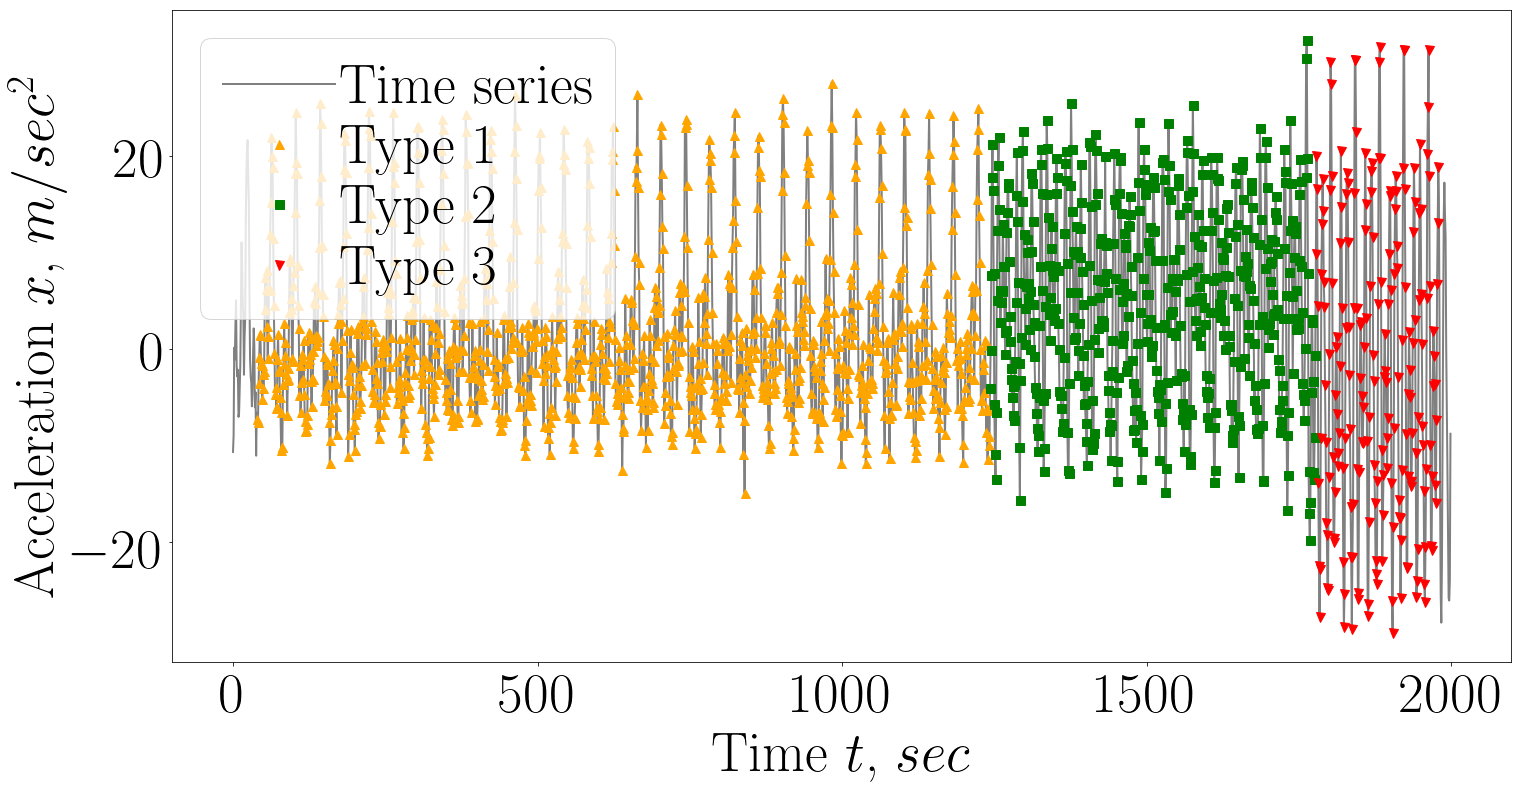
\includegraphics[width=0.5\textwidth]{results/3_patern_2_claster_vector}}\\
\caption{Кластеризация точек временного ряда: a) для временного ряда Synthetic~1; b) для временного ряда Synthetic~2}
\label{fig_synthetic_claster}
\end{figure}


\paragraph{Синтетические данные.}


На рис.~\ref{fig_synthetic_series} приведен пример синтетических временных рядов. 
На рис.~\ref{fig_synthetic_series_2} показан пример ряда в котором число различных сегментов~$K = 2$, а длина каждого сегмента~$T = 20$. 
На рис.~\ref{fig_synthetic_series_3} показан пример ряда в котором число различных сегментов~$K = 3$, а длина каждого сегмента~$T = 20$. 

Рис.~\ref{fig_synthetic_distance} иллюстрирует матрицы попарных расстояний~$\textbf{M}$ между всеми парами точек~$t$ временного ряда, которые построены при помощи~(\ref{eq:cl:9}). 
Используя матрицу попарных расстояний и метод Multidimensional Scaling~\cite{Borg2005} визуализируем точки временного ряда на плоскости. 
На рис.~\ref{fig_synthetic_2D} показана визуализация точек на плоскости и выполнена их кластеризация при помощи метода иерархической кластеризации. 
Иллюстрация кластеров точек временного ряда продемонстрирована на рис.~\ref{fig_synthetic_claster}.

\begin{figure}[h!t]\center
\subfloat[]
{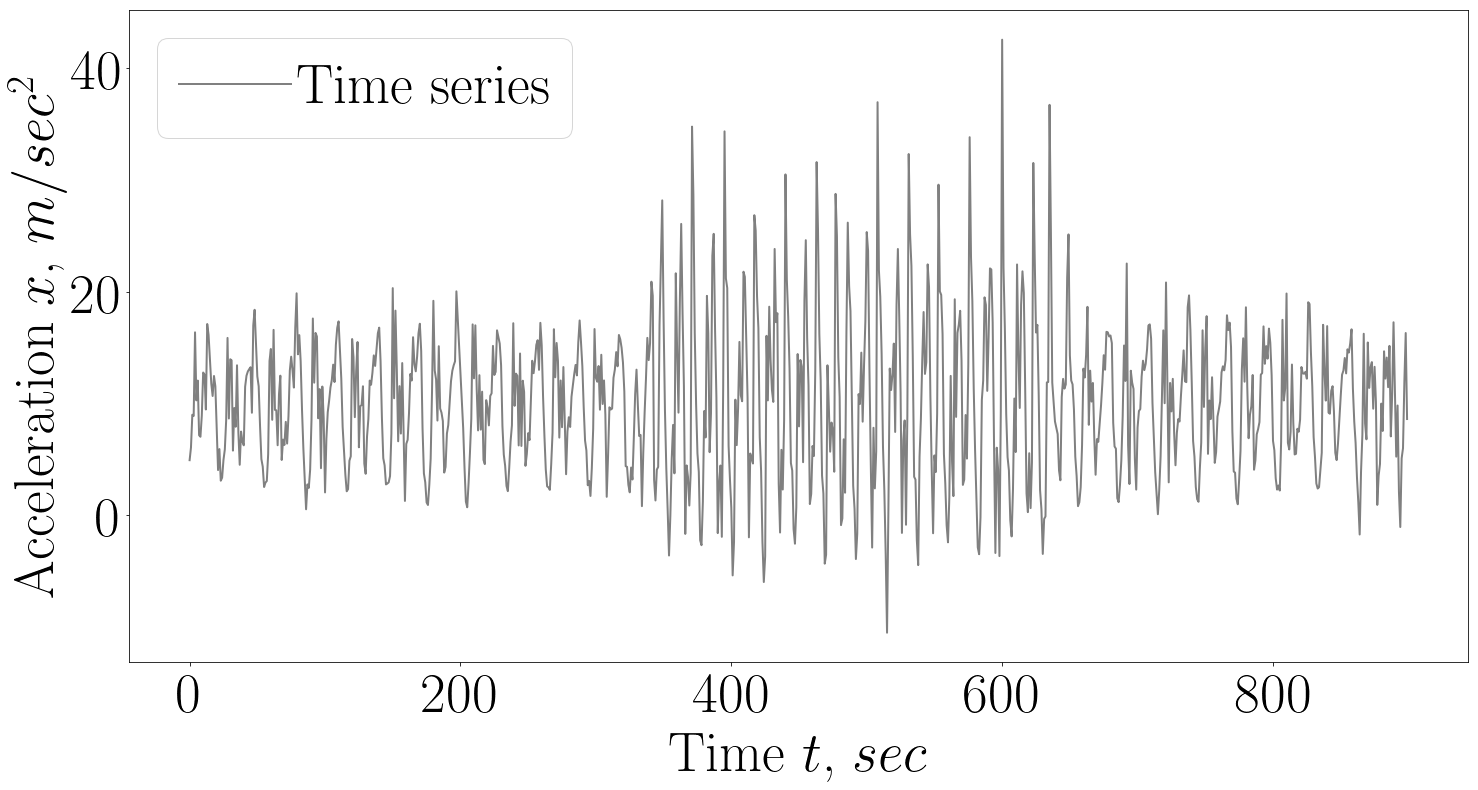
\includegraphics[width=0.5\textwidth]{results/real_1_series}}
\subfloat[]
{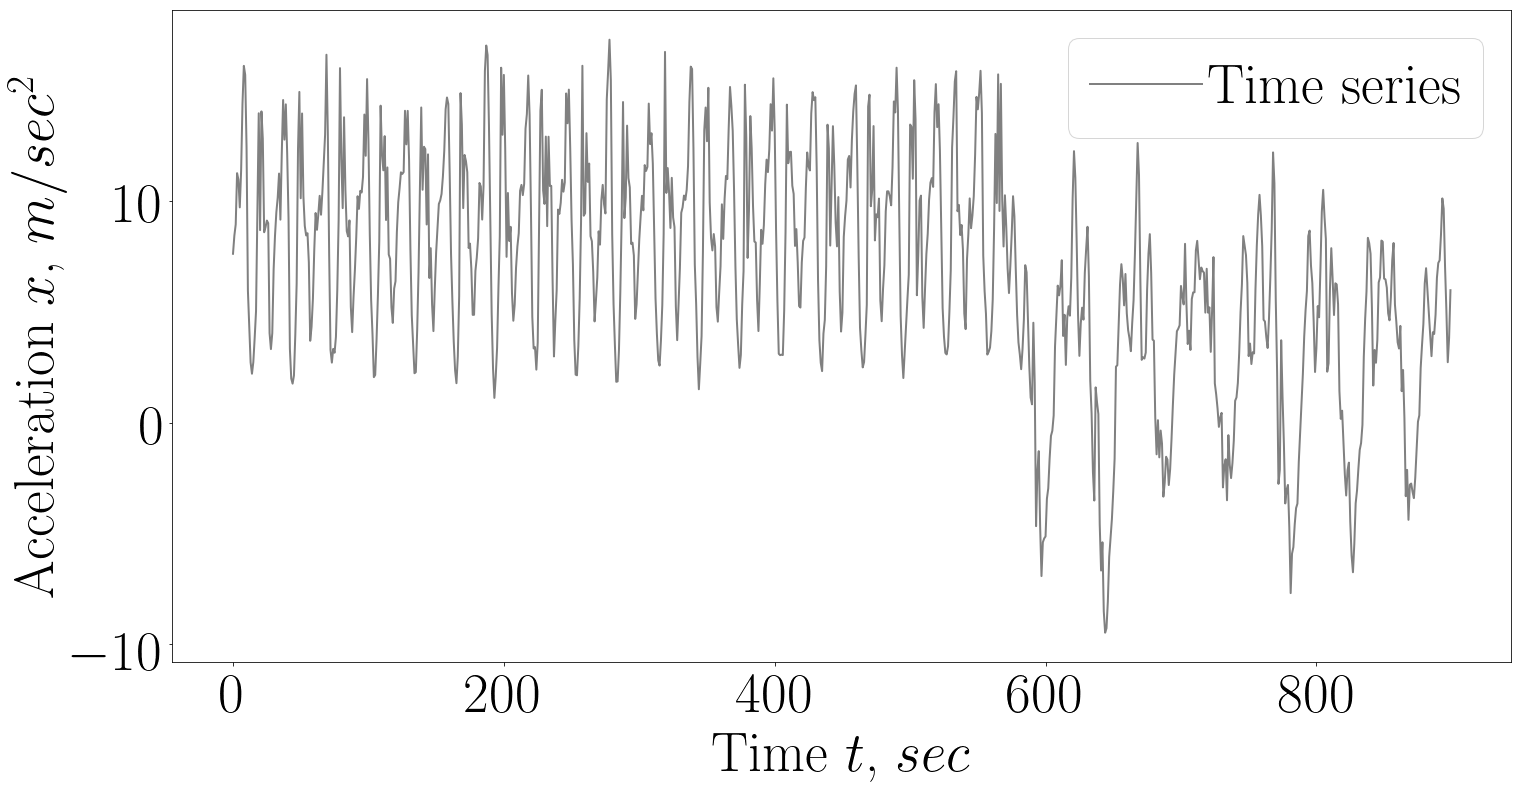
\includegraphics[width=0.5\textwidth]{results/real_2_series}}\\
\caption{Пример синтетически построенных временных рядов: a) для временного ряда Physical~Motion~1; b) для временного ряда Physical~Motion~2}
\label{fig_real_series}
\end{figure}

\begin{figure}[h!t]\center
\subfloat[]
{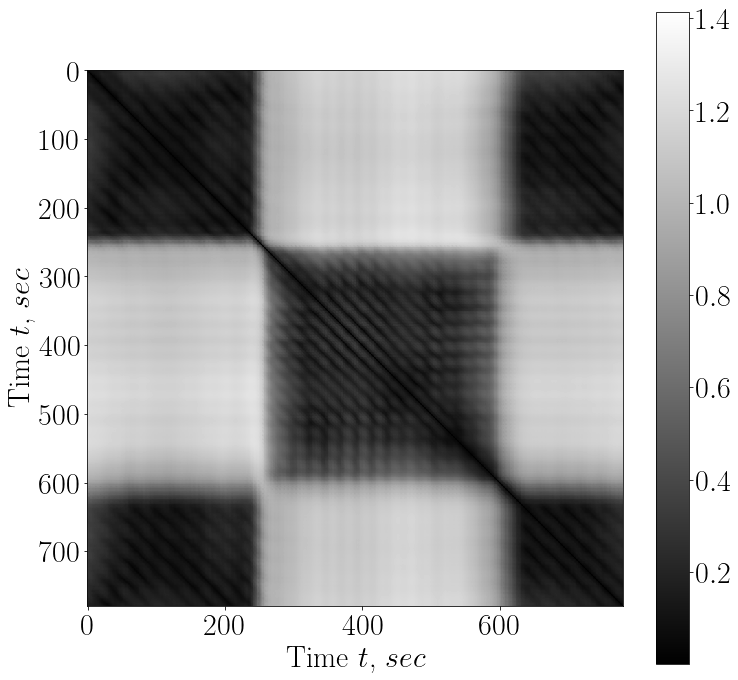
\includegraphics[width=0.5\textwidth]{results/real_1_full}}
\subfloat[]
{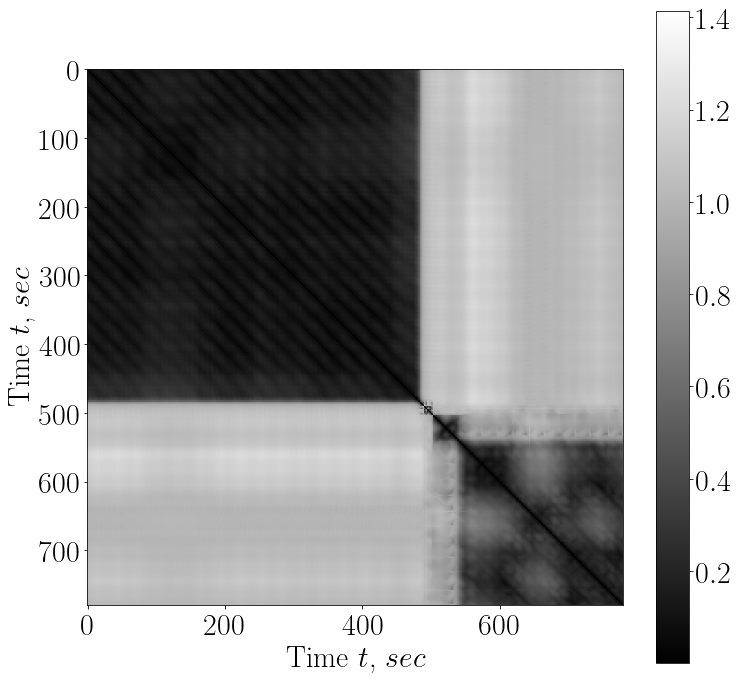
\includegraphics[width=0.5\textwidth]{results/real_2_full}}\\
\caption{Матрица попарных расстояний~$\textbf{M}$ между точками временного ряда: a) для временного ряда Physical~Motion~1; b) для временного ряда Physical~Motion~2}
\label{fig_real_distance}
\end{figure}

\begin{figure}[h!t]\center
\subfloat[]
{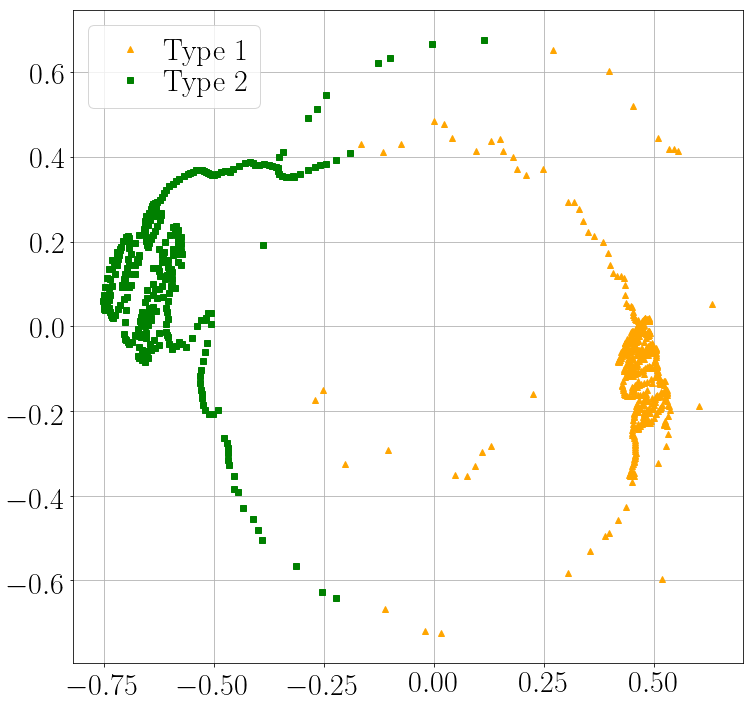
\includegraphics[width=0.5\textwidth]{results/real_1_2D_vector}}
\subfloat[]
{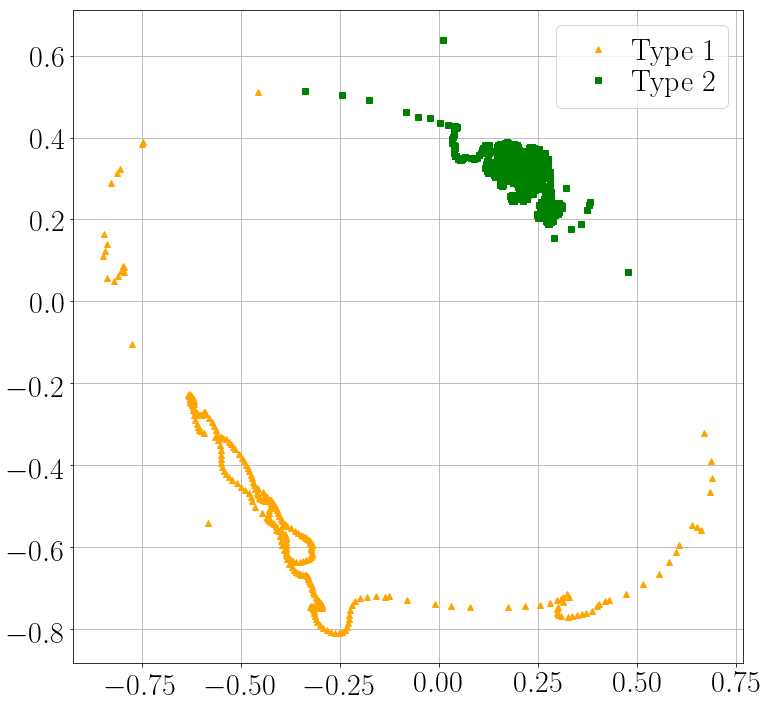
\includegraphics[width=0.5\textwidth]{results/real_2_2D_vector}}\\
\caption{Проекция точек временного на плоскость при помощи матрицы попарных расстояний~$\textbf{M}$: a) для временного ряда Physical~Motion~1; b) для временного ряда Physical~Motion~2}
\label{fig_real_2D}
\end{figure}

\begin{figure}[h!t]\center
\subfloat[]
{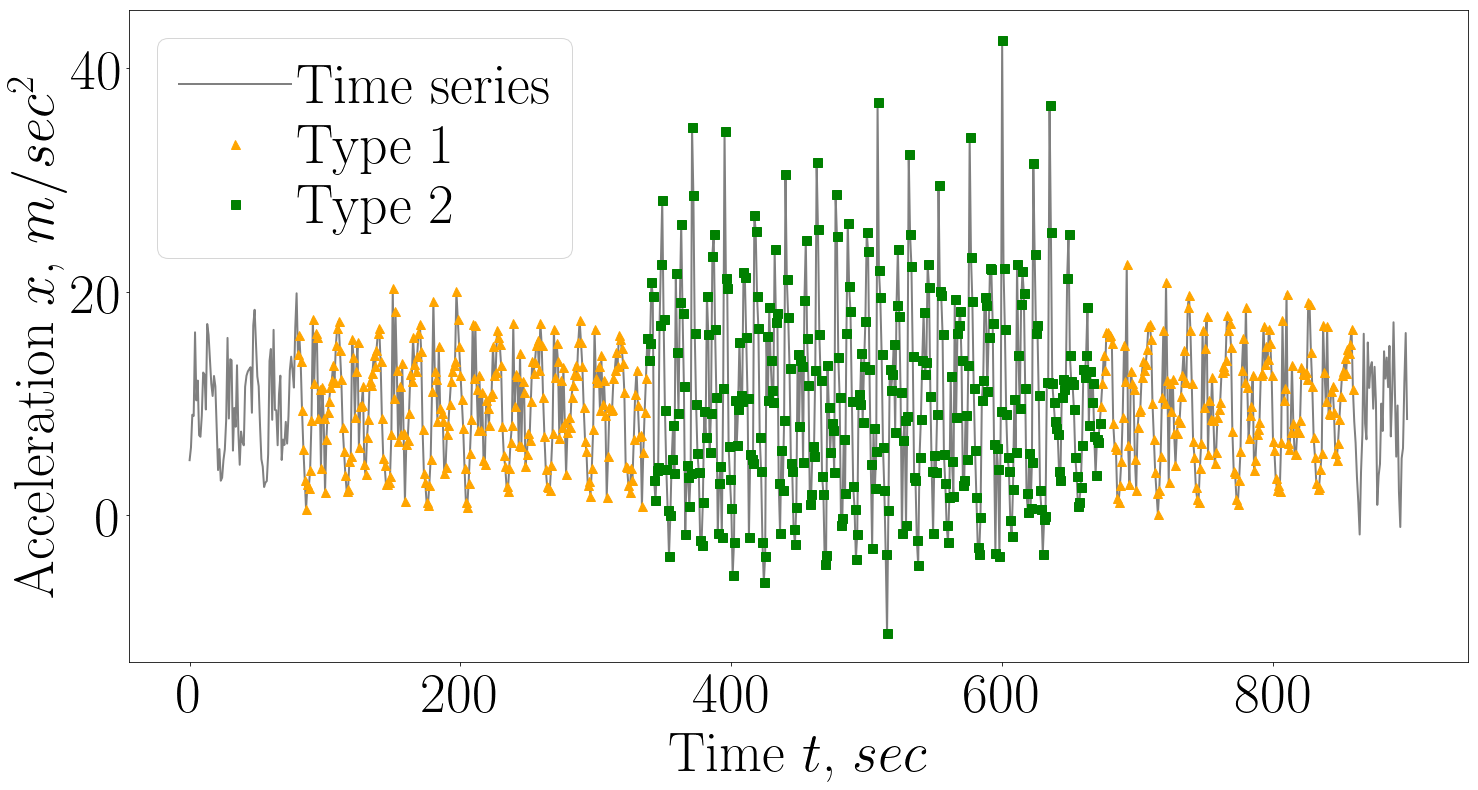
\includegraphics[width=0.5\textwidth]{results/real_1_claster_vector}}
\subfloat[]
{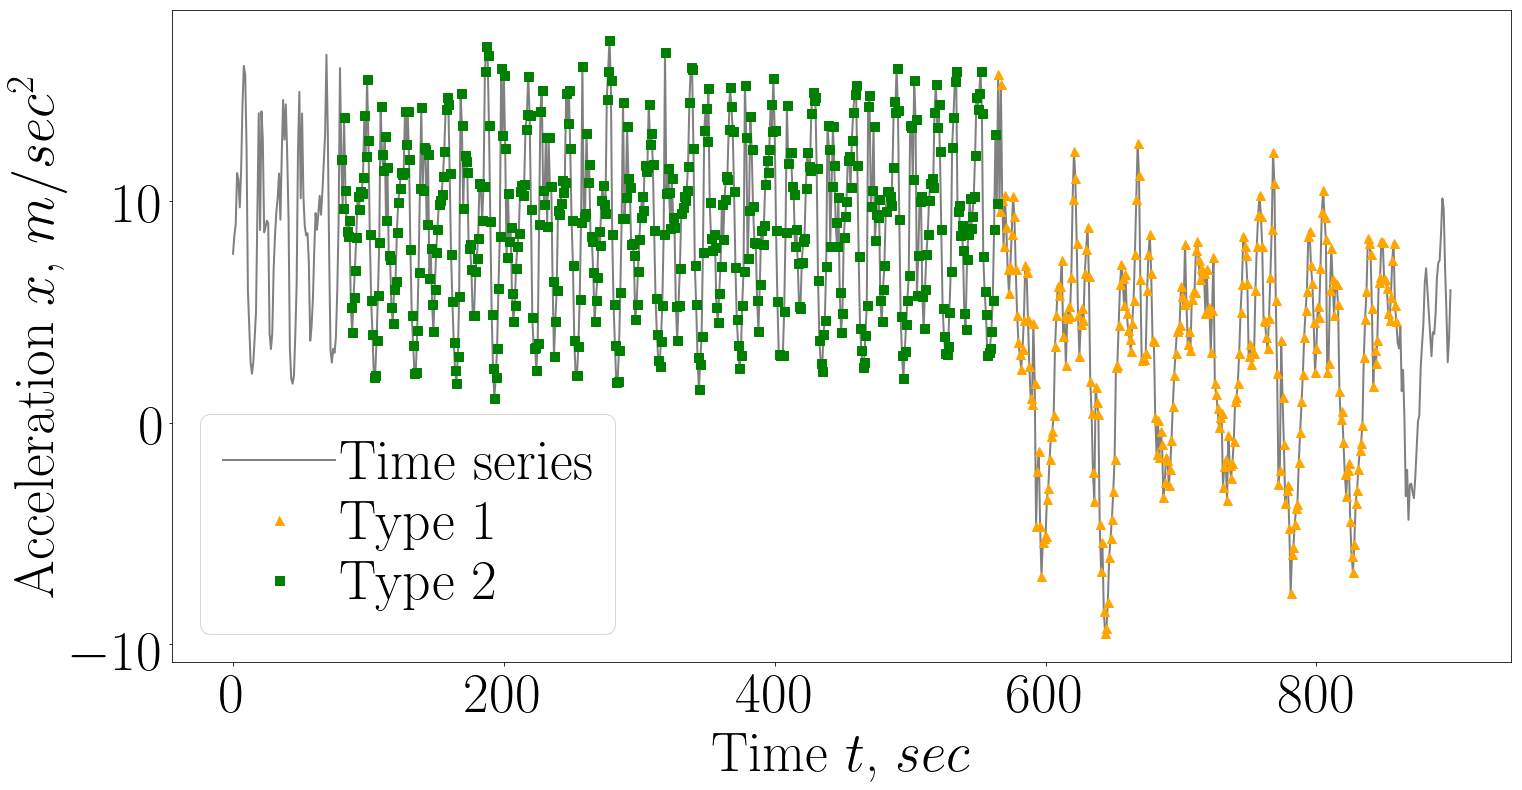
\includegraphics[width=0.5\textwidth]{results/real_2_claster_vector}}\\
\caption{Кластеризация точек временного ряда: 
a) для временного ряда Physical~Motion~1; b) для временного ряда Physical~Motion~2}
\label{fig_real_claster}
\end{figure}

\paragraph{Реальные данные.}

На рис.~\ref{fig_real_series} приведен пример реальных временных рядов полученных при помощи взятия одной из координат мобильного акселерометра. 

Рис.~\ref{fig_real_distance} иллюстрирует матрицы попарных расстояний~$\textbf{M}$ между всеми парами точек~$t$ временного ряда, которые построены при помощи~(\ref{eq:cl:9}). 
Используя матрицу попарных расстояний и метод Multidimensional Scaling~\cite{Borg2005} визуализируем точки временного ряда на плоскости. 
На рис.~\ref{fig_real_2D} показана визуализация точек на плоскости и выполнена их кластеризация при помощи метода иерархической кластеризации. 
Иллюстрация кластеров точек временного ряда продемонстрирована на рис.~\ref{fig_real_claster}.

\subsection{Сегментация временный рядов}
Сегментация временных рядов проводится на синтетических и реальных данных. Для данного эксперимента в качестве синтетического ряда рассматривается ряд построенный из двух синусов с произвольной частотой и амплитудой. Описание временных рядов, которые используются в данном эксперименте представлены в таблице~\ref{table:3}.

Сегментация проводится при помощи метода, который представлен в работе~\cite{motrenko2015}. Данный метод применяется для каждого действия внутри временного ряда по отдельности.


\begin{table}[h!t]
\begin{center}
\caption{Описание временных рядов в эксперименте сегментации временных рядов}
\label{table:3}
\begin{tabular}{|c|c|c|c|}
\hline
	Ряд,~$\textbf{x}$ &Длина ряда,~$N$& Число сегментов,~$K$&Длина сегмента,~$T$\\
	\hline
	\multicolumn{1}{|l|}{Simple~1}
	& 1000& 2& 100\\
	\hline
	\multicolumn{1}{|l|}{Physical~Motion~2}
	& 900& 2& 40\\
\hline

\end{tabular}
\end{center}
\end{table}

\paragraph{Синтетические данные.} На рис.~\ref{fig_simple_segmentation} показан результат работы сегментации для временного ряда Simple~1. 
Данный алгоритм хорошо выделил начала сегментов. 
Также на рис.~\ref{fig_simple_segmentation} показаны проекции фазовых пространств для обеих кластеров на их первые две главные компоненты.

\begin{figure}[h!t]\center
\subfloat[]
{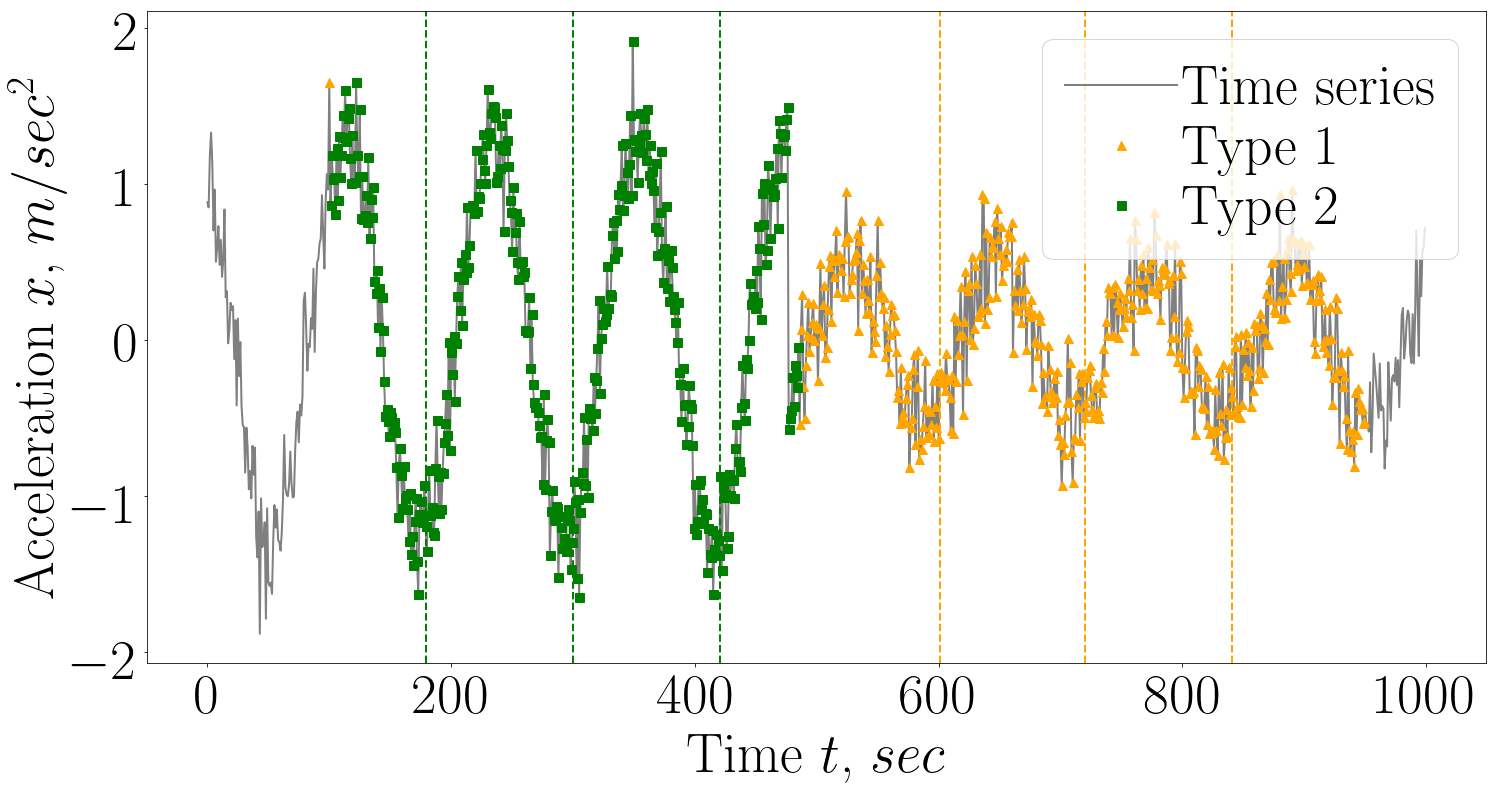
\includegraphics[width=0.5\textwidth]{results/simple_1_segmentation_vector}}
\subfloat[]
{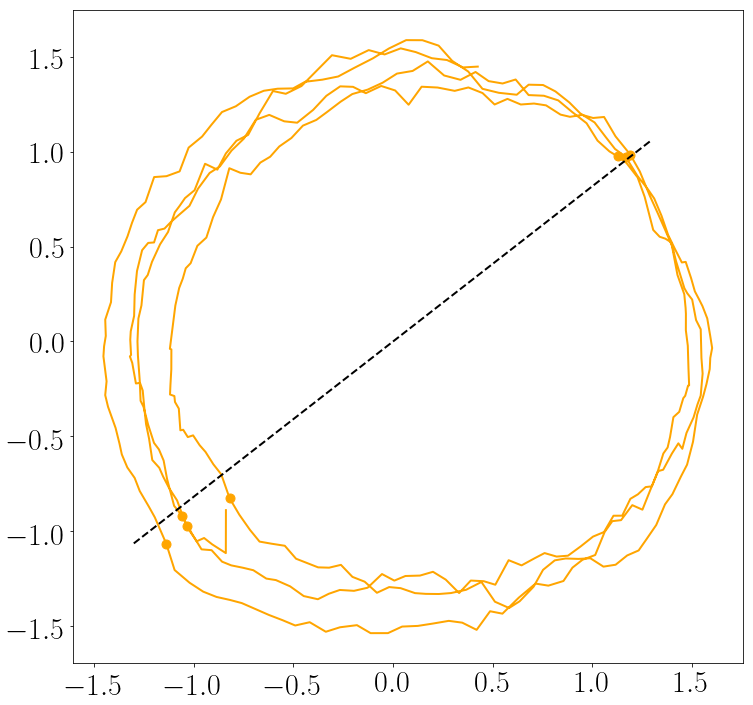
\includegraphics[width=0.25\textwidth]{results/simple_1_phase_space0}}
\subfloat[]
{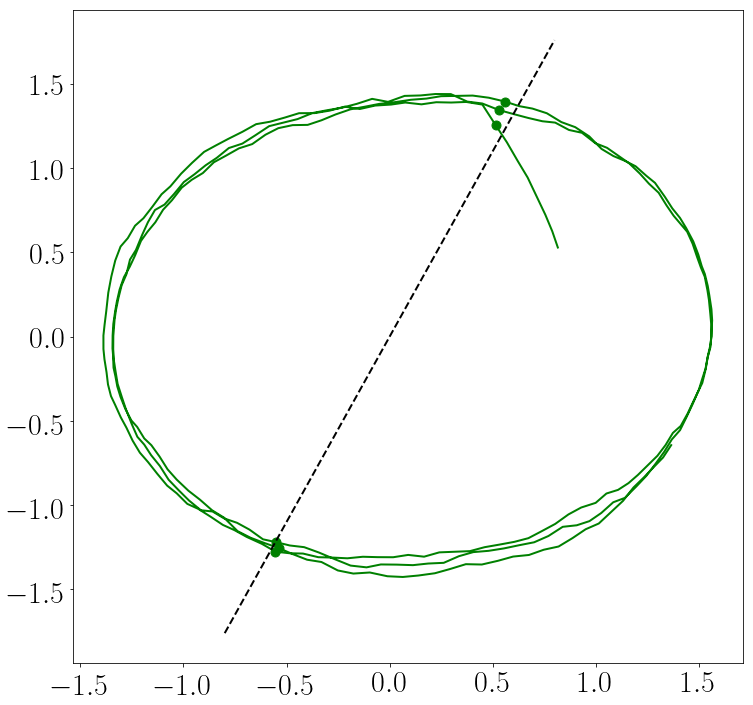
\includegraphics[width=0.25\textwidth]{results/simple_1_phase_space1}}\\
\caption{Сегментация точек временного ряда Simple~1: 
a) сегментация временного ряда; b) проекция фазового пространства на первые две главные компоненты для первого кластера; c) проекция фазового пространства на первые две главные компоненты для второго кластера}
\label{fig_simple_segmentation}
\end{figure}

\paragraph{Реальные данные.} На рис.~\ref{fig_real_segmentation} показан результат работы сегментации для временного ряда Physical~Motion~2. 
Данный алгоритм хорошо выделил начала сегментов для Type~1 и плохо для Type~2. 
Также на рис.~\ref{fig_real_segmentation} показаны проекции фазовых пространств для обеих кластеров на их первые две главные компоненты. 
Видно, что в случае проекции фазового пространства для части ряда, который относится к Type~2 получаем, что фазовая траектория имеет самопересечение внутри одного сегмента, что влечет нахождения ложного начала сегмента.

\begin{figure}[h!t]\center
\subfloat[]
{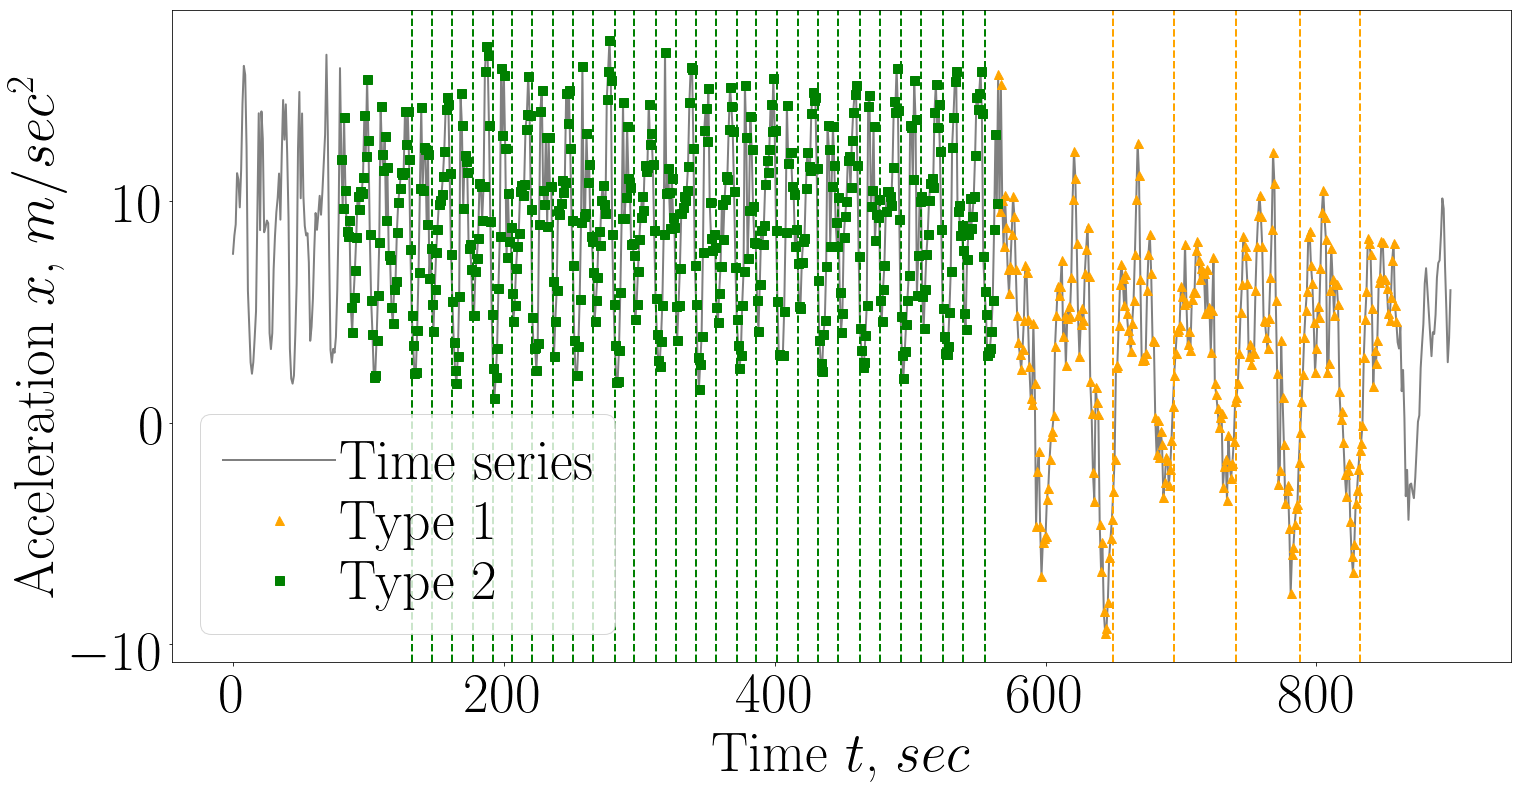
\includegraphics[width=0.5\textwidth]{results/real_2_segmentation_vector}}
\subfloat[]
{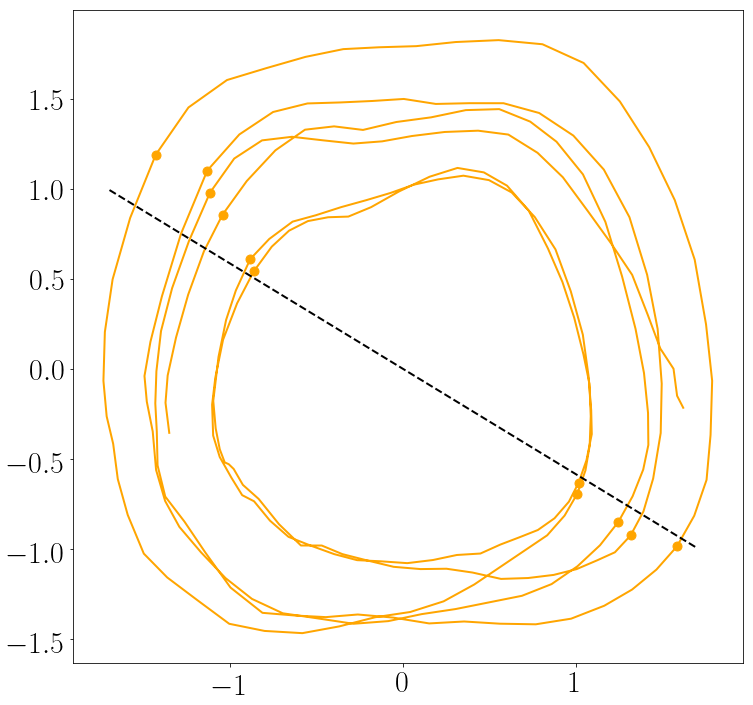
\includegraphics[width=0.25\textwidth]{results/real_2_phase_space0}}
\subfloat[]
{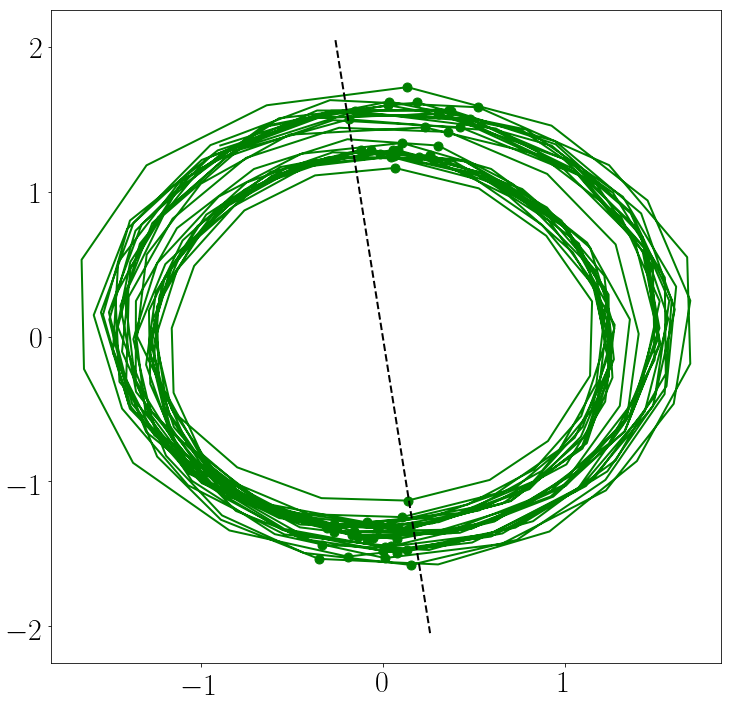
\includegraphics[width=0.25\textwidth]{results/real_2_phase_space1}}\\
\caption{Сегментация точек временного ряда Physical~Motion~2: 
a) сегментация временного ряда; b) проекция фазового пространства на первые две главные компоненты для первого кластера; c) проекция фазового пространства на первые две главные компоненты для второго кластера}
\label{fig_real_segmentation}
\end{figure}
